\documentclass[11pt,a4paper]{article}
\usepackage[T1]{fontenc}
\usepackage[utf8]{inputenc}
\usepackage[english]{babel}
\babelprovide[main,import]{slovenian}
\usepackage{lmodern}
\usepackage[margin=2.5cm]{geometry}
\usepackage{graphicx}
\usepackage{float}
\usepackage{enumitem}
\usepackage[hidelinks]{hyperref}
\usepackage{url}

\setlist{itemsep=2pt,topsep=4pt}

\title{\textbf{Pregled obstoječih rešitev}\\[4pt]
\large Projekt: spletna trgovina Pixel Corner}
\author{Anže \and Nejc \and Domen Arnuš}
\date{Komuniciranje in delo v skupinah, november 2026}

\begin{document}
\maketitle

\section{Uvod}

Naša skupina izdeluje spletno stran za trgovino Pixel Corner. Prodajala bo video igre, konzole in dodatke, posebej pa retro opremo: stare konzole, kot sta SNES in PlayStation 1, igre zanje ter krmilnike.

Problem, ki ga rešujemo, je precej preprost. Kdor v Sloveniji išče originalno retro konzolo ali igro, ima na izbiro predvsem oglase na Bolhi in tuje trgovine z dragim pošiljanjem. Pri oglasih ne veš, ali stvar sploh deluje. Pri večjih domačih trgovinah pa je \glqq retro\grqq{} ponavadi le poceni mini konzola z že naloženimi igrami. Radi bi naredili stran, kjer je rabljena oprema pregledana, jasno opisana in jo je mogoče hitro najti po platformi.

Preden smo začeli risati svoje zaslone, smo pregledali tri obstoječe trgovine: CeX, GameStop in Big Bang. Pri vsaki nas je zanimalo, kako je urejen katalog, kako so opisani rabljeni izdelki in kaj nas pri uporabi moti.

\section{Obstoječe rešitve}

\subsection{CeX (webuy.com)}

CeX je britanska veriga, ki kupuje, prodaja in menja rabljeno tehniko, med drugim igre, konzole in telefone \cite{cex}. Začela je leta 1992 kot ena sama trgovina z igrami, danes pa ima več kot 600 poslovalnic v več kot desetih državah \cite{cex-zgodovina}. Na spletni strani je zbrana zaloga vseh njihovih trgovin, med njo tudi retro konzole, kot je Super Nintendo \cite{cex-clanek}.

\textbf{Ključne funkcionalnosti:}
\begin{itemize}
  \item nakup rabljenih in novih iger, konzol in dodatkov, tudi retro,
  \item prodaja lastnih stvari: uporabnik poišče izdelek, izbere stanje in takoj dobi ponudbo v gotovini ali kot dobropis \cite{cex-prodaja},
  \item ocene stanja (od A do F) in več različic iste konzole (s škatlo, brez škatle, znižano) \cite{cex-clanek},
  \item 5-letna garancija na elektroniko in vračilo spletnih naročil v 14 dneh \cite{cex} (slika~\ref{fig:cex}),
  \item rezervacija prek spleta in prevzem v trgovini (Click \& Collect) \cite{cex-zgodovina}.
\end{itemize}

\textbf{Prednosti:} zelo velika izbira, stanje izdelka je jasno označeno z oceno, garancija velja tudi za rabljeno opremo, cene so pregledne.

\textbf{Slabosti:} v Sloveniji ne posluje. Uporabniki se v ocenah pritožujejo, da spletna naročila in odkup trajajo predolgo in da so jim naročila preklicali, ker izdelka ni bilo na zalogi \cite{cex-ocene}. Stran prodaja vse, od telefonov do filmov, zato je igre treba posebej iskati.

\begin{figure}[H]
  \centering
  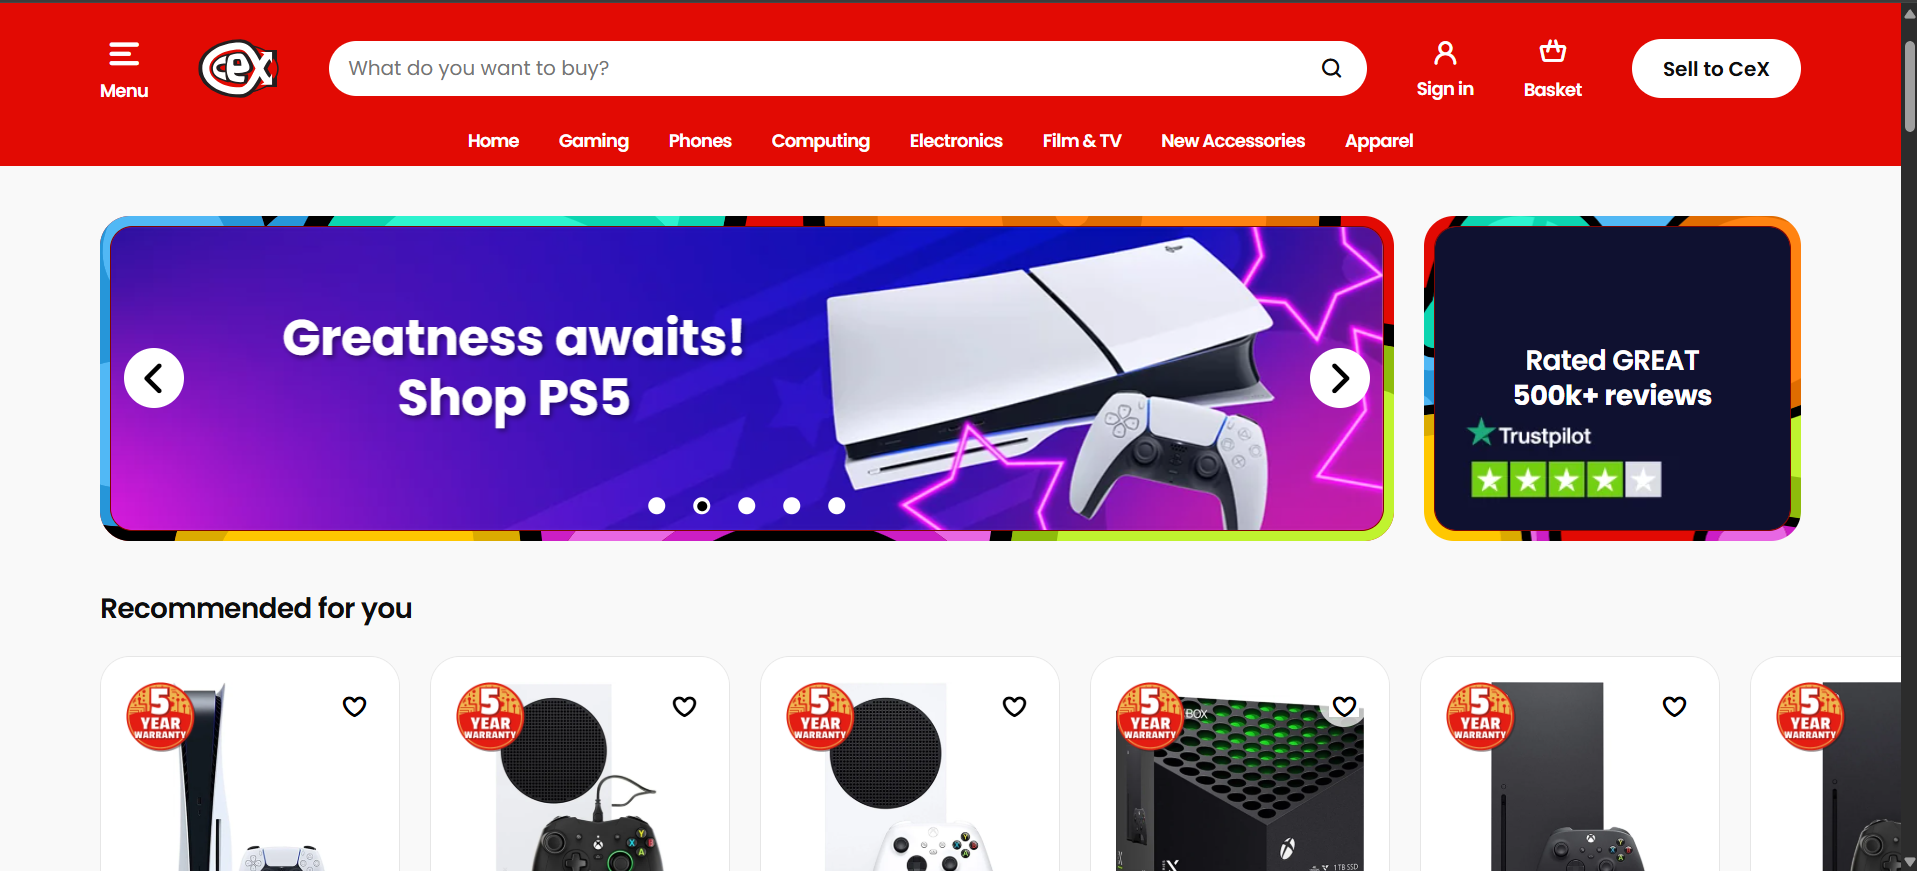
\includegraphics[width=0.9\textwidth]{cex.png}
  \caption{Domača stran CeX z gumbom \glqq Sell to CeX\grqq{} in oznako 5-letne garancije na izdelkih.}
  \label{fig:cex}
\end{figure}

\subsection{GameStop (retro kategorija)}

GameStop je ameriška trgovina z igrami. Na svoji strani ima posebno kategorijo Retro Gaming z več kot deset tisoč izdelki, večinoma rabljenimi \cite{gamestop}.

\textbf{Ključne funkcionalnosti:}
\begin{itemize}
  \item filtri po platformi (Game Boy, Nintendo 64, PlayStation 2 \ldots), stanju (novo ali rabljeno), žanru in ceni \cite{gamestop},
  \item razvrščanje po ceni, priljubljenosti in datumu izida,
  \item izbira dostave: na dom, isti dan ali prevzem v trgovini,
  \item odkup starih iger (Trade-In) in program zvestobe.
\end{itemize}

\textbf{Prednosti:} filtri so zelo natančni, retro ponudba je ločena od ostale in ima svojo pasico z logotipi platform (slika~\ref{fig:gamestop}). To nam je bilo najbolj všeč. Seznam izdelkov je pregleden in vsaka kartica ima sliko, ceno in platformo.

\textbf{Slabosti:} dostava le v ZDA. Glavni meni je prenatrpan (igre, zbirateljske kartice, oblačila \ldots), med izdelki pa so tudi sponzorirani zadetki, ki zmotijo. Pri rabljenih izdelkih je opis stanja kratek.

\begin{figure}[H]
  \centering
  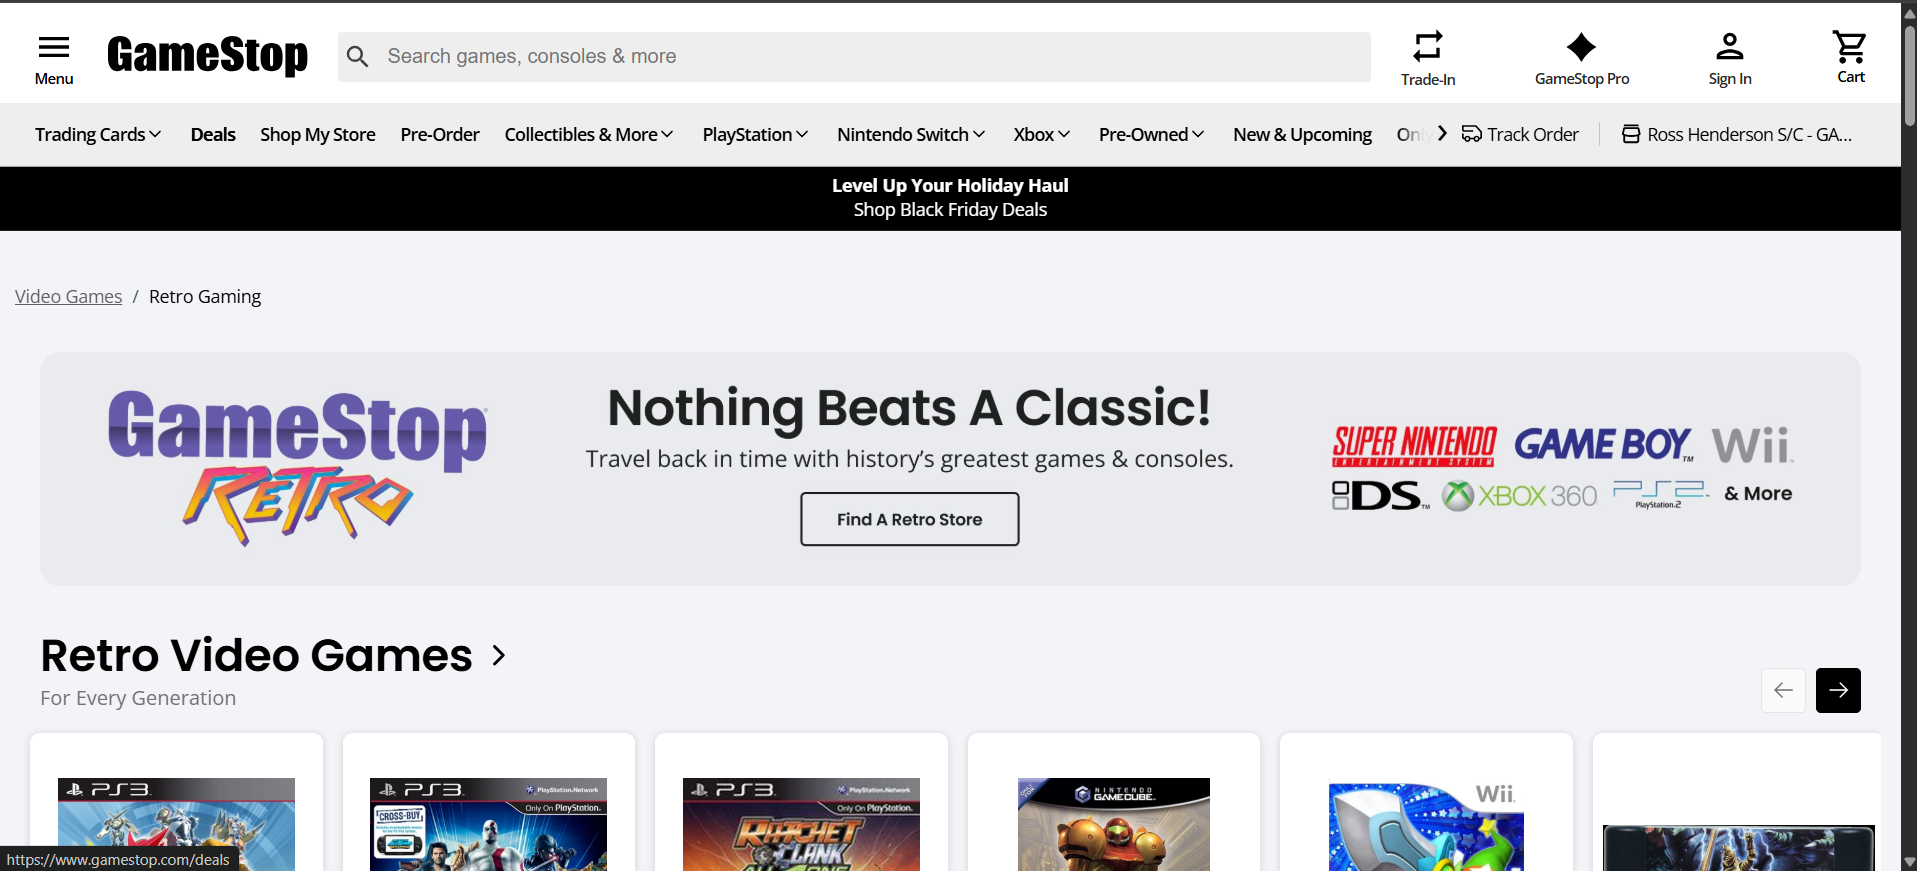
\includegraphics[width=0.9\textwidth]{gamestop.png}
  \caption{Kategorija Retro Gaming na strani GameStop.}
  \label{fig:gamestop}
\end{figure}

\subsection{Big Bang}

Big Bang je slovenska trgovina z elektroniko, ki ima tudi kategorijo za gaming: konzole PlayStation, Xbox in Nintendo, opremo zanje in igre \cite{bigbang-gaming}. Retro ponudba so predvsem mini konzole z več tisoč že naloženimi igrami, na primer M8 Mini \cite{bigbang-m8}.

\textbf{Ključne funkcionalnosti:}
\begin{itemize}
  \item spletna prodaja z dostavo po Sloveniji in prevzemom v poslovalnicah,
  \item kategorije in podkategorije (konzole, oprema, igre),
  \item filtri po ceni, blagovni znamki in zalogi v poslovalnici, akcijske cene (slika~\ref{fig:bigbang}),
  \item stran izdelka s slikami, opisom in specifikacijami.
\end{itemize}

\textbf{Prednosti:} vse je v slovenščini, dostava je hitra, cene so v evrih in trgovine so blizu. Stran je urejena in znana večini kupcev.

\textbf{Slabosti:} gaming je le majhen del ponudbe med televizorji in gospodinjskimi aparati. Rabljene in originalne retro opreme ni. Opisi retro izdelkov so pogosto kar prepisani iz angleščine.

\begin{figure}[H]
  \centering
  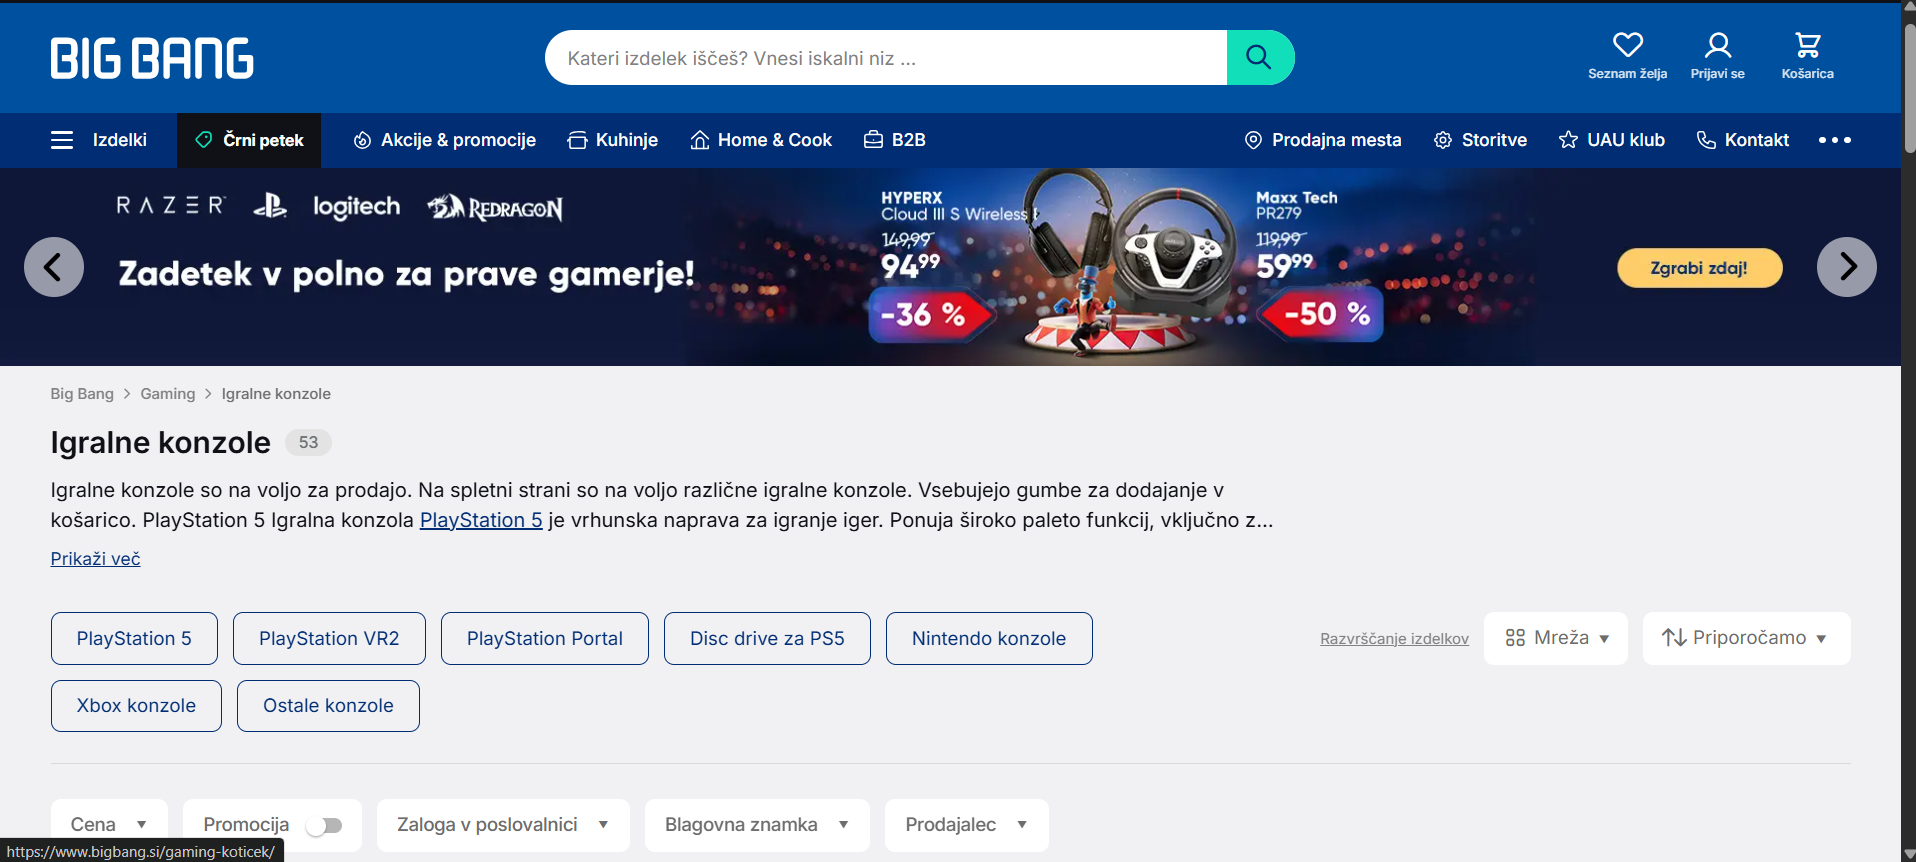
\includegraphics[width=0.9\textwidth]{bigbang.png}
  \caption{Kategorija Igralne konzole v trgovini Big Bang s podkategorijami in filtri.}
  \label{fig:bigbang}
\end{figure}

\section{Zaključek}

Od GameStopa bomo vzeli filtre po platformi in stanju ter ločeno retro kategorijo. Od CeX-a bomo vzeli jasno oznako stanja rabljenega izdelka, od Big Banga pa preprosto stran izdelka in slovenski jezik.

Naša stran bo drugačna v treh stvareh. Prvič, prodajala bo samo igre in gaming opremo, zato bo meni kratek in ne bo treba iskati med telefoni in pralnimi stroji. Drugič, pri vsakem rabljenem izdelku bo pisalo, ali je testiran, ali ima originalno škatlo in kakšno je ohišje. Tretjič, retro opremo, ki je CeX in GameStop v Sloveniji ne ponujata, bomo prodajali v slovenščini, cene bodo v evrih, dostava pa po Sloveniji. Prve verzije bodo imele domačo stran, trgovino s filtri, stran izdelka, košarico in kontakt. Blagajno dodamo kasneje.

\begin{thebibliography}{9}
\bibitem{cex} CeX / WeBuy UK, \emph{Pregled storitev in pogojev}. Dostopno na: \url{https://uk.webuy.com/llms.txt} (dostopano 23.~11.~2026).
\bibitem{cex-zgodovina} Stockland, \emph{CeX -- Stockland Burleigh Heads}. Dostopno na: \url{https://stockland.com.au/shopping-centres/centres/stockland-burleigh-heads/stores/cex} (dostopano 23.~11.~2026).
\bibitem{cex-clanek} inkl, \emph{The joy of CeX: how to spend £10 in the secondhand gaming mega-store}. Dostopno na: \url{https://inkl.com/news/the-joy-of-cex-how-to-spend-10-in-the-secondhand-gaming-mega-store} (dostopano 23.~11.~2026).
\bibitem{cex-prodaja} Tech Insider, \emph{Where to sell your old console in Ireland}. Dostopno na: \url{https://tech-insider.org/ie/?p=1394} (dostopano 23.~11.~2026).
\bibitem{cex-ocene} Trustpilot, \emph{CeX/WeBuy -- United Kingdom: ocene uporabnikov}. Dostopno na: \url{https://ie.trustpilot.com/review/webuy.com?page=4} (dostopano 23.~11.~2026).
\bibitem{gamestop} GameStop, \emph{Retro Gaming}. Dostopno na: \url{https://www.gamestop.com/video-games/retro-gaming} (dostopano 23.~11.~2026).
\bibitem{bigbang-gaming} Nabava.net, \emph{Big Bang igraće konzole i video igre}. Dostopno na: \url{https://www.nabava.net/big-bang/ponuda?k=36} (dostopano 23.~11.~2026).
\bibitem{bigbang-m8} Big Bang, \emph{M8 Mini Video Game Console}. Dostopno na: \url{https://bigbang.si/m8-mini-video-game-console-4k-hd-10-000-games-in-1-wireless-handheld-retro-classic-gaming-for-tv-64gb-izdelek-1092966} (dostopano 23.~11.~2026).
\end{thebibliography}

\end{document}
